\documentclass[uplatex]{jsarticle}
\usepackage{listings, jlisting}
\lstset{
  basicstyle={\ttfamily},
  identifierstyle={\small},
  commentstyle={\smallitshape},
  keywordstyle={\small\bfseries},
  ndkeywordstyle={\small},
  stringstyle={\small\ttfamily},
  frame={tb},
  breaklines=true,
  columns=[l]{fullflexible},
  numbers=left,
  xrightmargin=0zw,
  xleftmargin=3zw,
  numberstyle={\scriptsize},
  stepnumber=1,
  numbersep=1zw,
  lineskip=-0.5ex
}
\usepackage[dvipdfmx]{graphicx}
\title{データベース2 課題}

\author{101730153 佐治 礼仁 saji.ayahito@h.mbox.nagoya-u.ac.jp}
\date{\today}
\begin{document}
\maketitle
\section{実行環境}
\begin{itemize}
  \item MySQL Server version: 8.0.18 MySQL Community Server
\end{itemize}
\section{解答}
\subsection{問1}
問1のSQLをソースコード\ref{lst:sql1}に,実行結果を図\ref{fig:ans1}に示す.
\begin{lstlisting}[caption=問1のSQL,label=lst:sql1]
SELECT 部門名 FROM 部門 NATURAL JOIN 従業員 WHERE 氏名="山田一郎";
\end{lstlisting}
\begin{figure}[htb]
\begin{center}
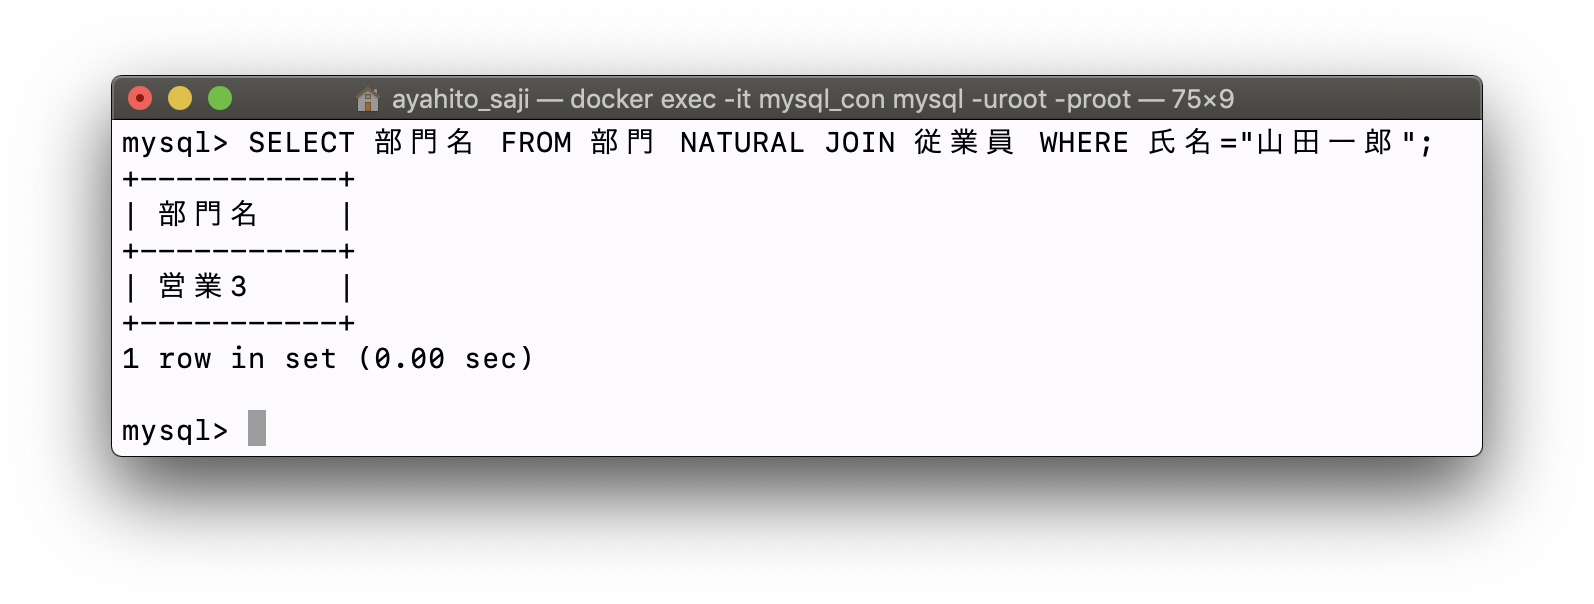
\includegraphics[width=100mm]{figures/ans1.png}
\caption{問1の実行結果}
\label{fig:ans1}
\end{center}
\end{figure}

\subsection{問2}
問2のSQLをソースコード\ref{lst:sql2}に,実行結果を図\ref{fig:ans2}に示す.
\begin{lstlisting}[caption=問2のSQL,label=lst:sql2]
SELECT DISTINCT 部門番号, 部門名 FROM 部門 NATURAL JOIN 従業員 WHERE 年齢<20;
\end{lstlisting}
\begin{figure}[htb]
\begin{center}
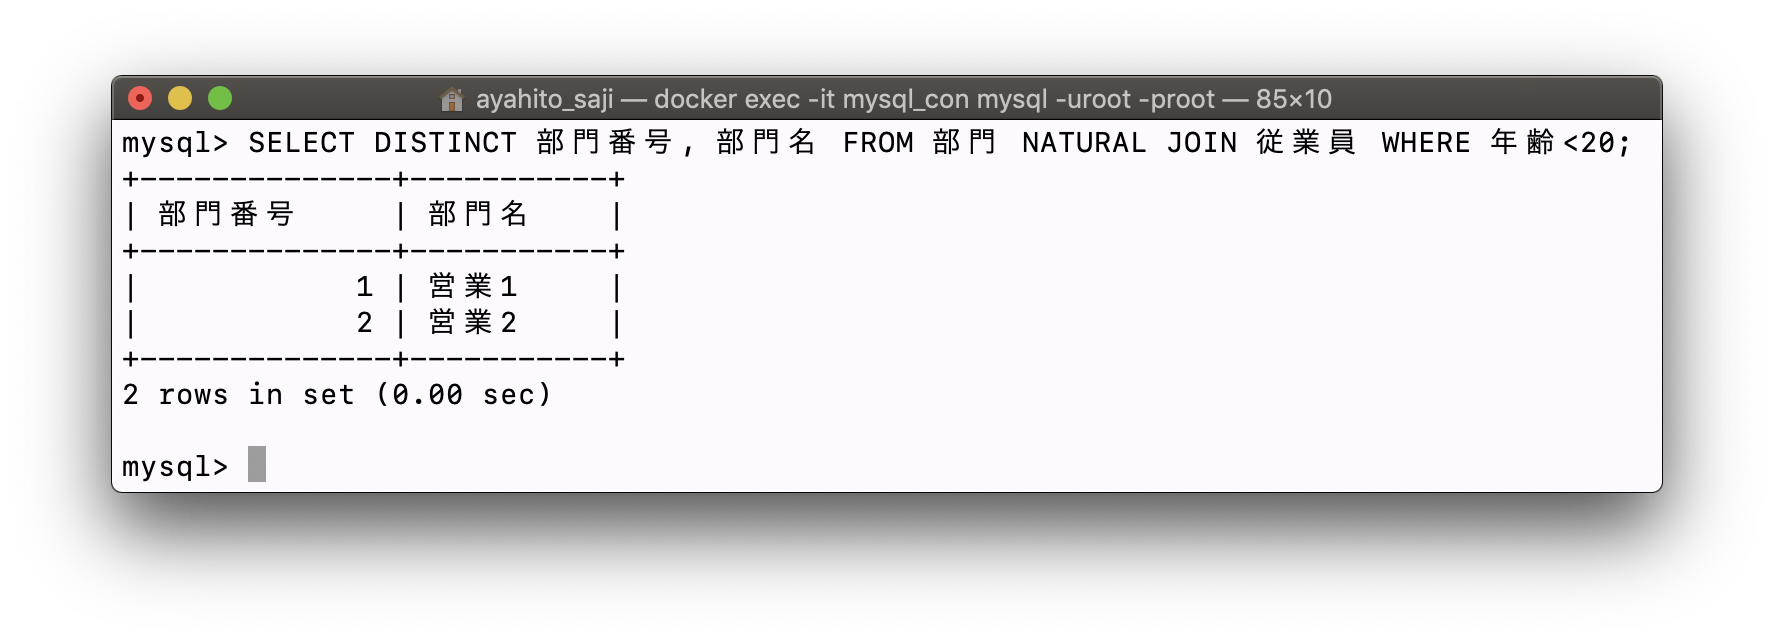
\includegraphics[width=100mm]{figures/ans2.png}
\caption{問2の実行結果}
\label{fig:ans2}
\end{center}
\end{figure}

\subsection{問3}
問3のSQLをソースコード\ref{lst:sql3}に,実行結果を図\ref{fig:ans3}に示す.
\begin{lstlisting}[caption=問3のSQL,label=lst:sql3]
SELECT 業者番号 FROM 供給 WHERE 部品番号=1 AND 単価<(SELECT 単価 FROM 供給 WHERE 部品番号=1 AND 業者番号=3 AND 部門番号=2);
\end{lstlisting}
\begin{figure}[htb]
\begin{center}
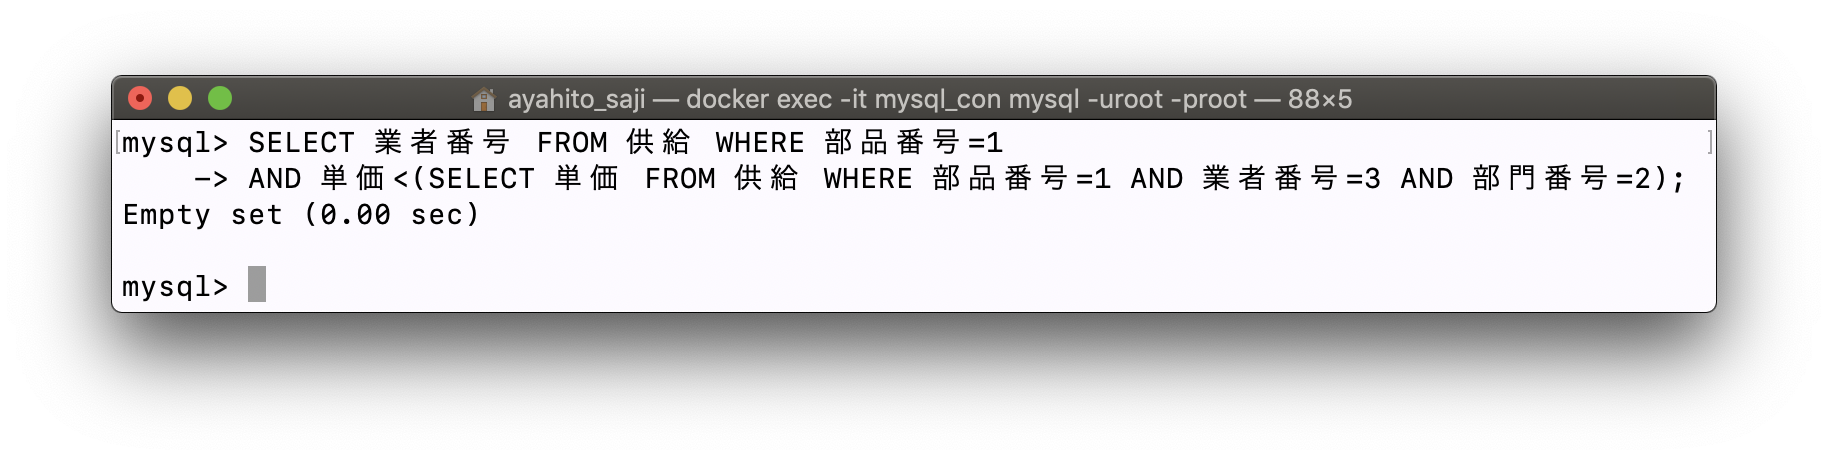
\includegraphics[width=120mm]{figures/ans3.png}
\caption{問3の実行結果}
\label{fig:ans3}
\end{center}
\end{figure}

\subsection{問4}
問4のSQLをソースコード\ref{lst:sql4}に,実行結果を図\ref{fig:ans4}に示す.
\begin{lstlisting}[caption=問4のSQL,label=lst:sql4]
SELECT 部門番号, 部門名 FROM 部門 AS X WHERE NOT EXISTS (SELECT * FROM 従業員 WHERE 年齢<20 AND X.部門番号=部門番号);
\end{lstlisting}
\begin{figure}[htb]
\begin{center}
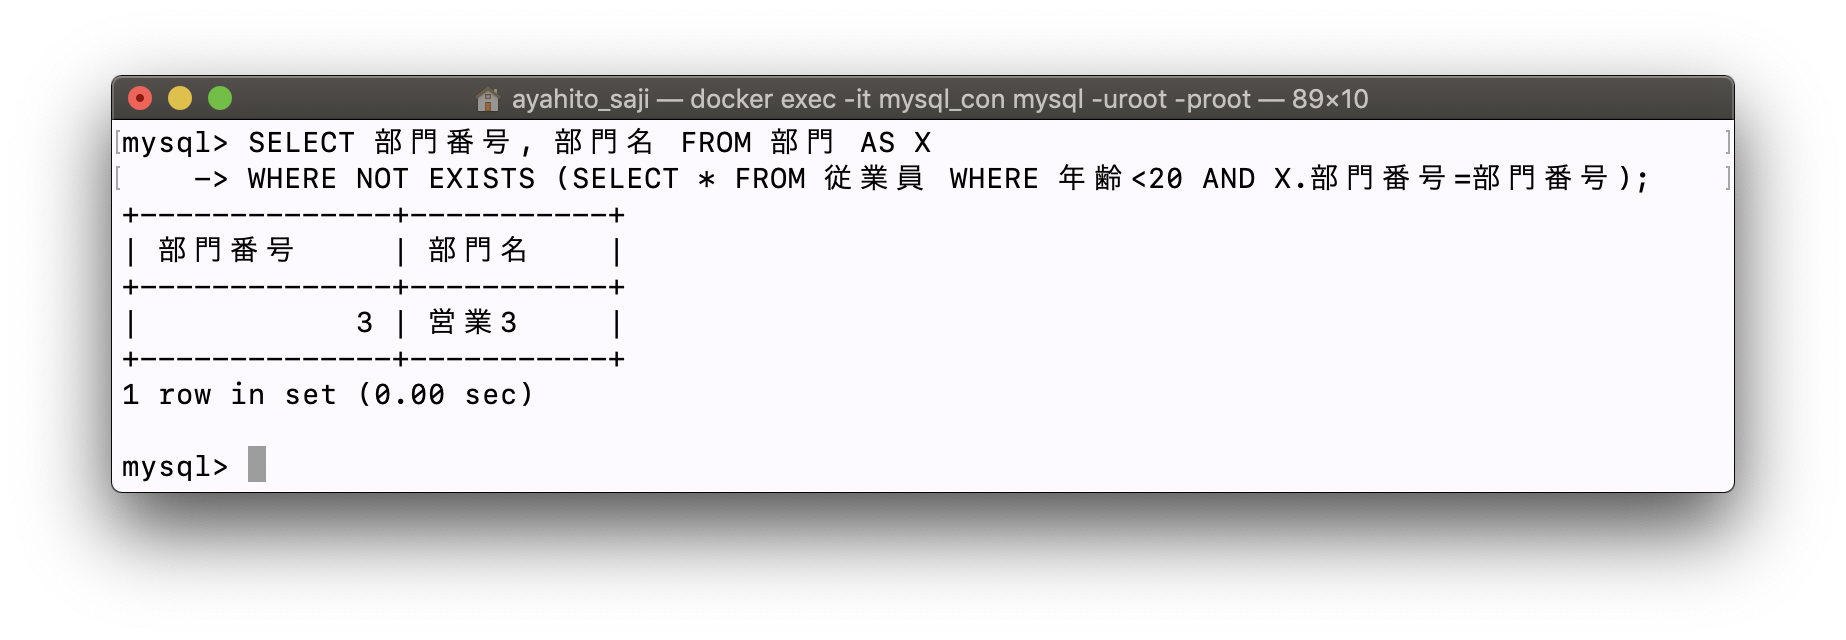
\includegraphics[width=100mm]{figures/ans4.png}
\caption{問4の実行結果}
\label{fig:ans4}
\end{center}
\end{figure}

\subsection{問5}
問5のSQLをソースコード\ref{lst:sql5}に,実行結果を図\ref{fig:ans5}に示す.
\begin{lstlisting}[caption=問5のSQL,label=lst:sql5]
SELECT COUNT(*) FROM 従業員 WHERE 部門番号=1;
\end{lstlisting}
\begin{figure}[htb]
\begin{center}
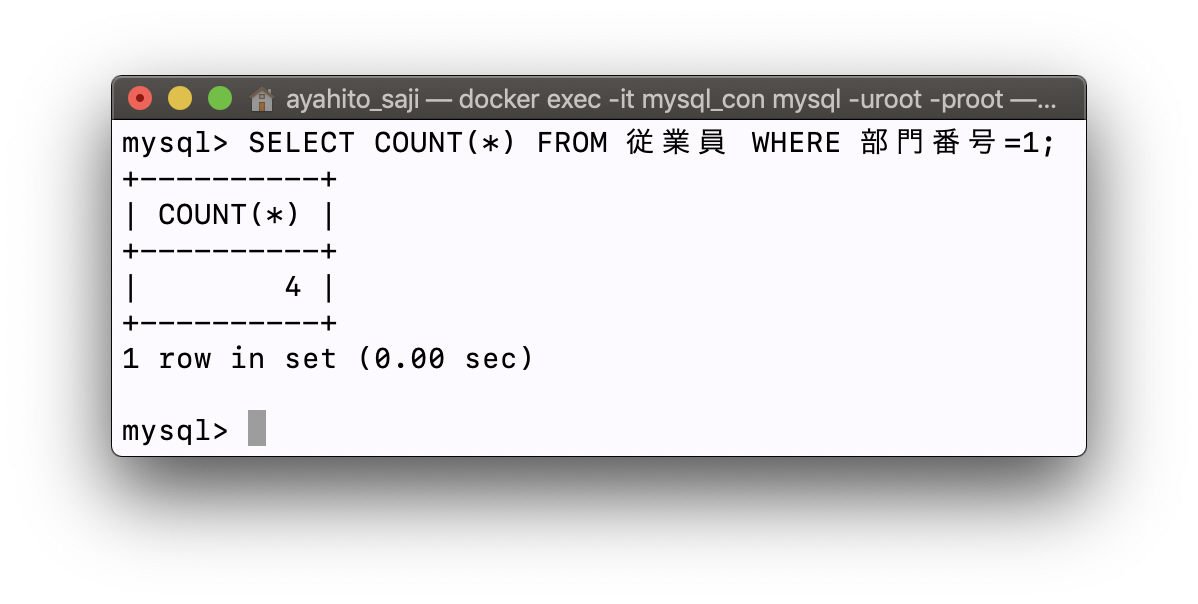
\includegraphics[width=100mm]{figures/ans5.png}
\caption{問5の実行結果}
\label{fig:ans5}
\end{center}
\end{figure}

\subsection{問6}
問6のSQLをソースコード\ref{lst:sql6}に,実行結果を図\ref{fig:ans6}に示す.
\begin{lstlisting}[caption=問6のSQL,label=lst:sql6]
SELECT 部門番号, COUNT(*) FROM 従業員 GROUP BY 部門番号;
\end{lstlisting}
\begin{figure}[htb]
\begin{center}
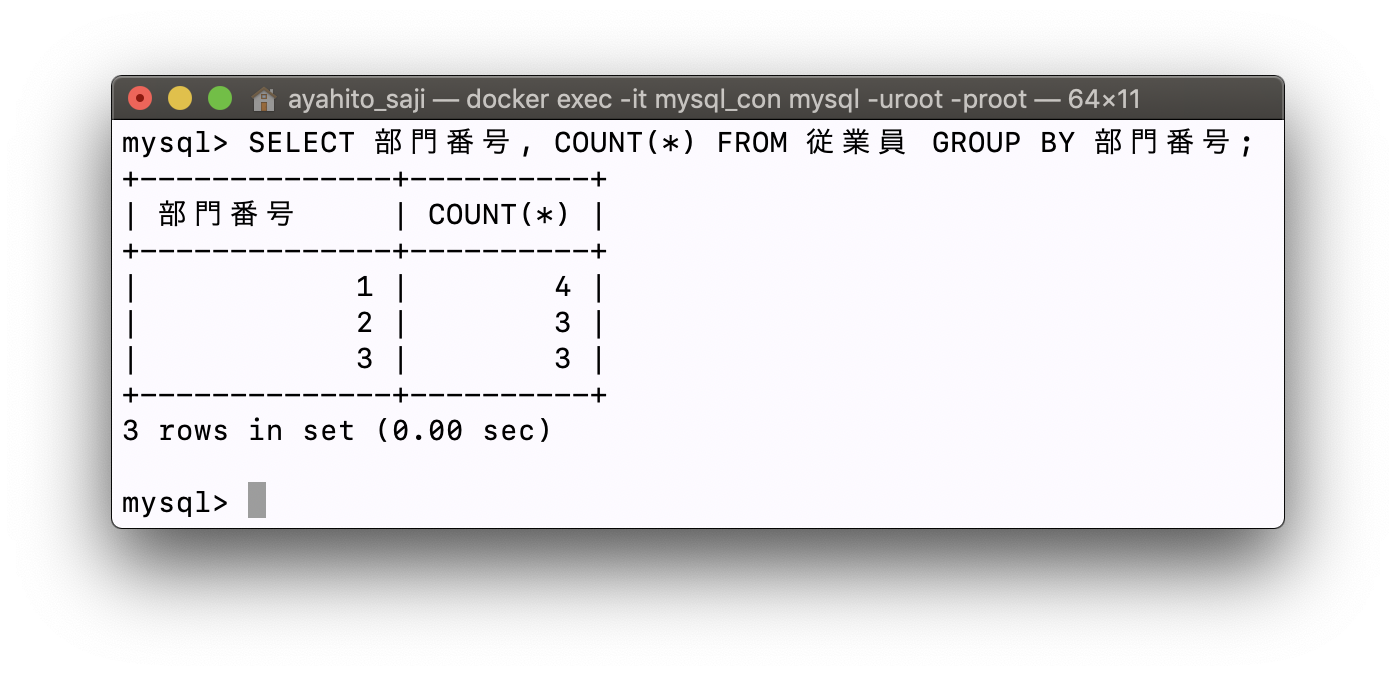
\includegraphics[width=100mm]{figures/ans6.png}
\caption{問6の実行結果}
\label{fig:ans6}
\end{center}
\end{figure}

\subsection{問7}
問7のSQLをソースコード\ref{lst:sql7}に,実行結果を図\ref{fig:ans7}に示す.
\begin{lstlisting}[caption=問7のSQL,label=lst:sql7]
SELECT 部品番号, MIN(単価), MAX(単価), AVG(単価) FROM 供給 GROUP BY 部品番号;
\end{lstlisting}
\begin{figure}[htb]
\begin{center}
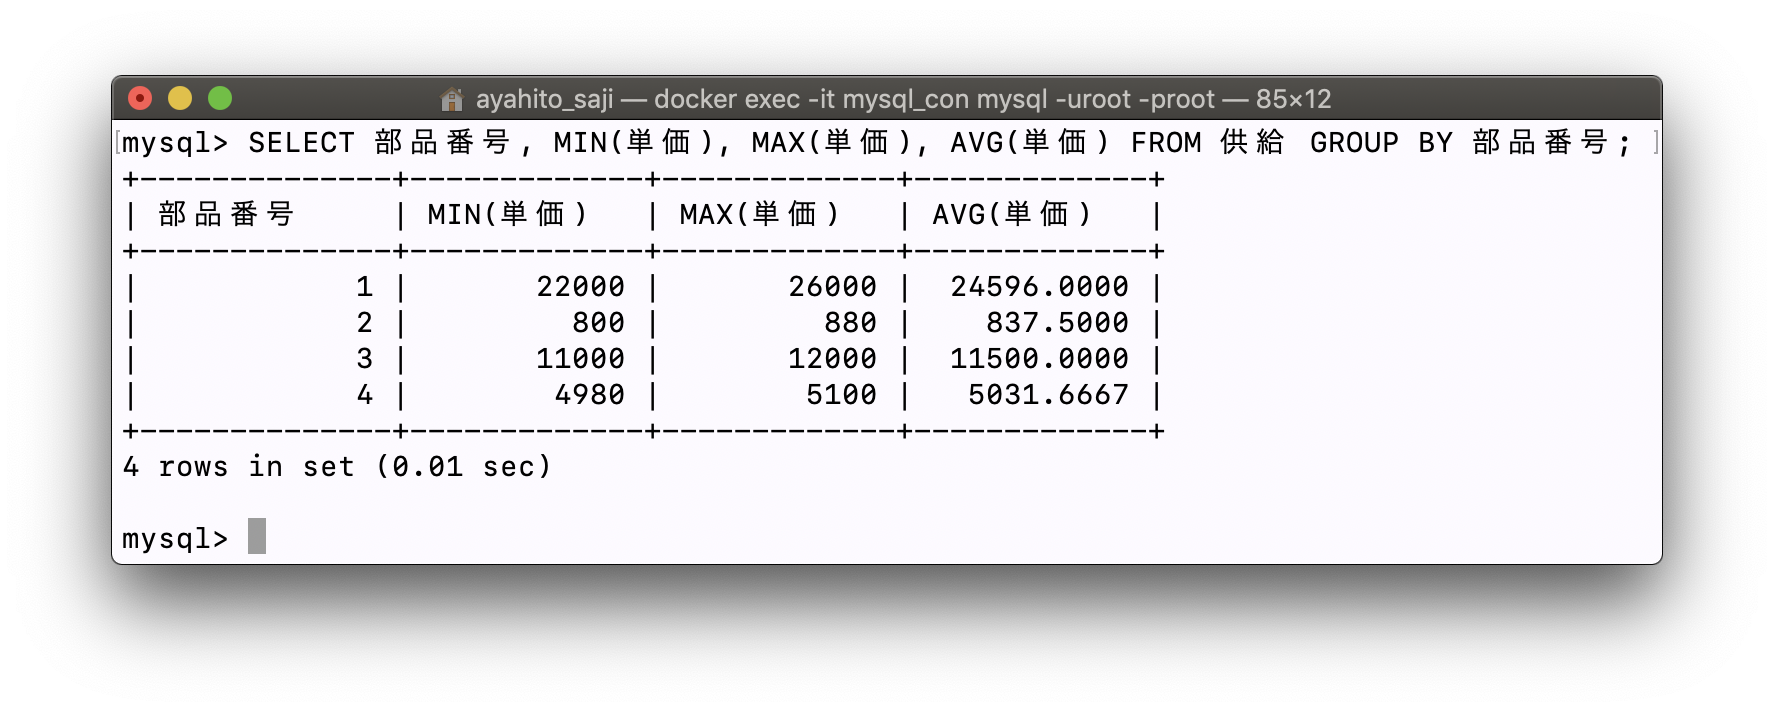
\includegraphics[width=100mm]{figures/ans7.png}
\caption{問7の実行結果}
\label{fig:ans7}
\end{center}
\end{figure}

\subsection{問8}
問8のSQLをソースコード\ref{lst:sql8}に,実行結果を図\ref{fig:ans8}に示す.
\begin{lstlisting}[caption=問8のSQL,label=lst:sql8]
SELECT DISTINCT 部品番号, 部品名 FROM 供給 NATURAL JOIN 部品 AS X WHERE (SELECT MAX(単価)-MIN(単価) FROM 供給 WHERE 部品番号=X.部品番号)>100;
\end{lstlisting}
\begin{figure}[htb]
\begin{center}
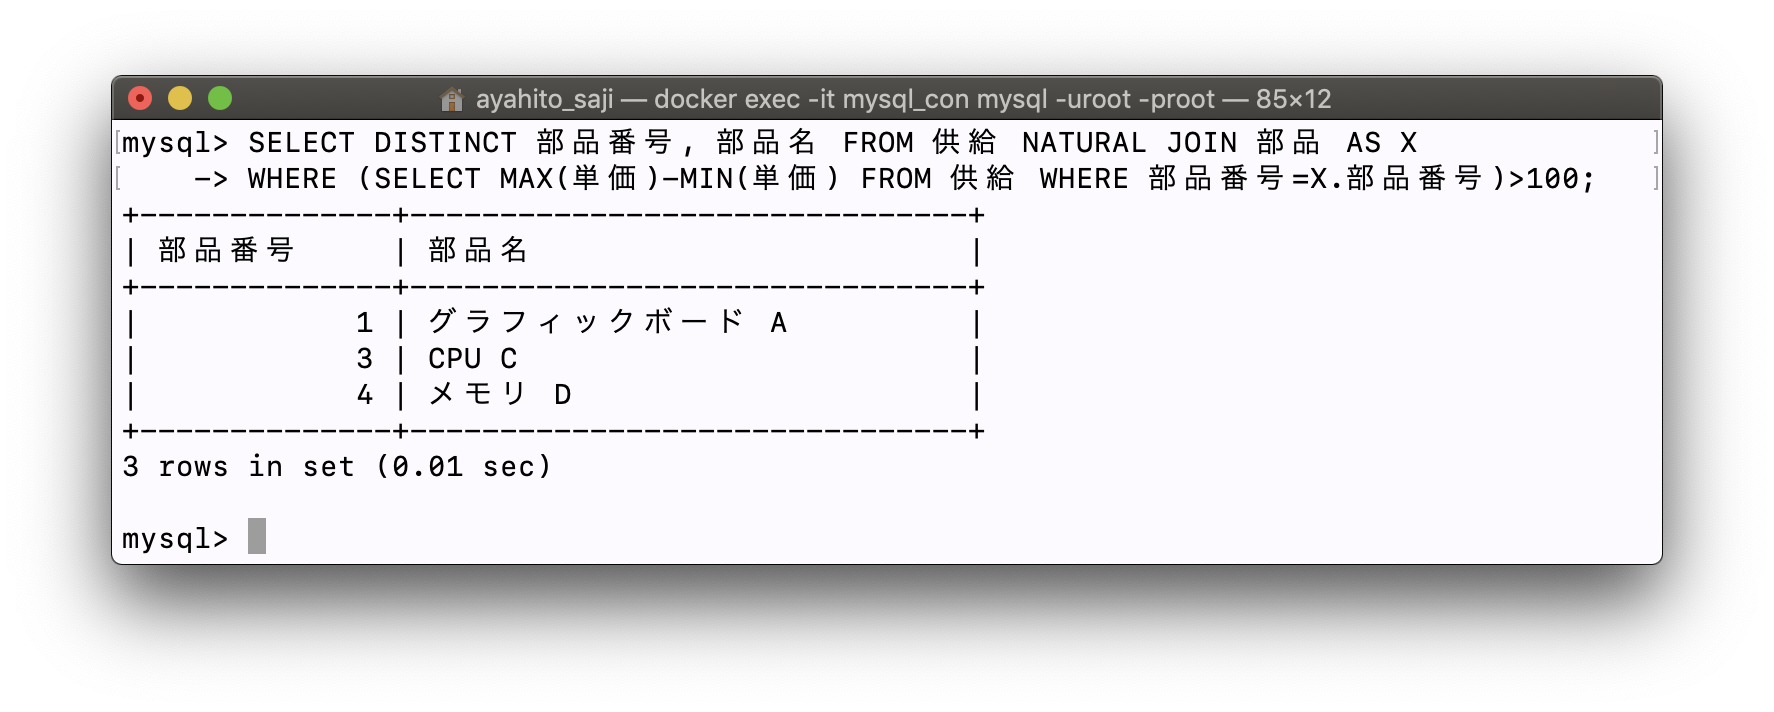
\includegraphics[width=100mm]{figures/ans8.png}
\caption{問8の実行結果}
\label{fig:ans8}
\end{center}
\end{figure}

\subsection{問9}
問9のSQLをソースコード\ref{lst:sql9}に,実行結果を図\ref{fig:ans9}に示す.
\begin{lstlisting}[caption=問9のSQL,label=lst:sql9]
SELECT 部品番号, MIN(単価), MAX(単価), AVG(単価) FROM 供給 WHERE 部門番号=1 GROUP BY 部品番号;
\end{lstlisting}
\begin{figure}[htb]
\begin{center}
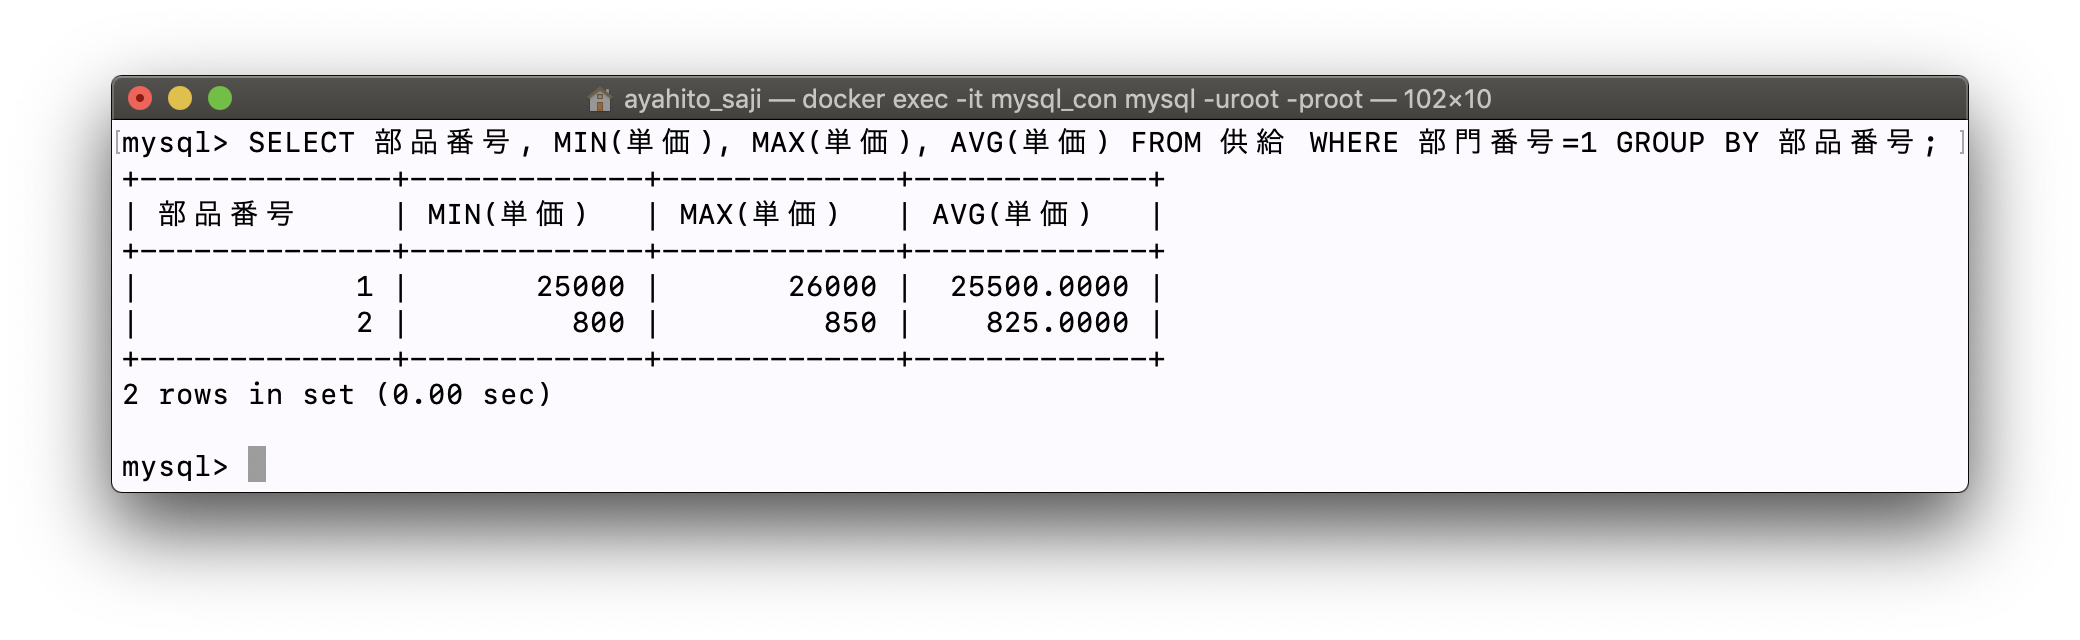
\includegraphics[width=120mm]{figures/ans9.png}
\caption{問9の実行結果}
\label{fig:ans9}
\end{center}
\end{figure}

\subsection{問10}
問10のSQLをソースコード\ref{lst:sql10}に,実行結果を図\ref{fig:ans10}に示す.
\begin{lstlisting}[caption=問10のSQL,label=lst:sql10]
SELECT * FROM (SELECT DISTINCT 部品番号 FROM 供給 WHERE 部門番号=1 ) AS X NATURAL JOIN (SELECT 部品番号, MIN(単価), MAX(単価), AVG(単価) FROM 供給 GROUP BY 部品番号) AS Y;
\end{lstlisting}
\begin{figure}[htb]
\begin{center}
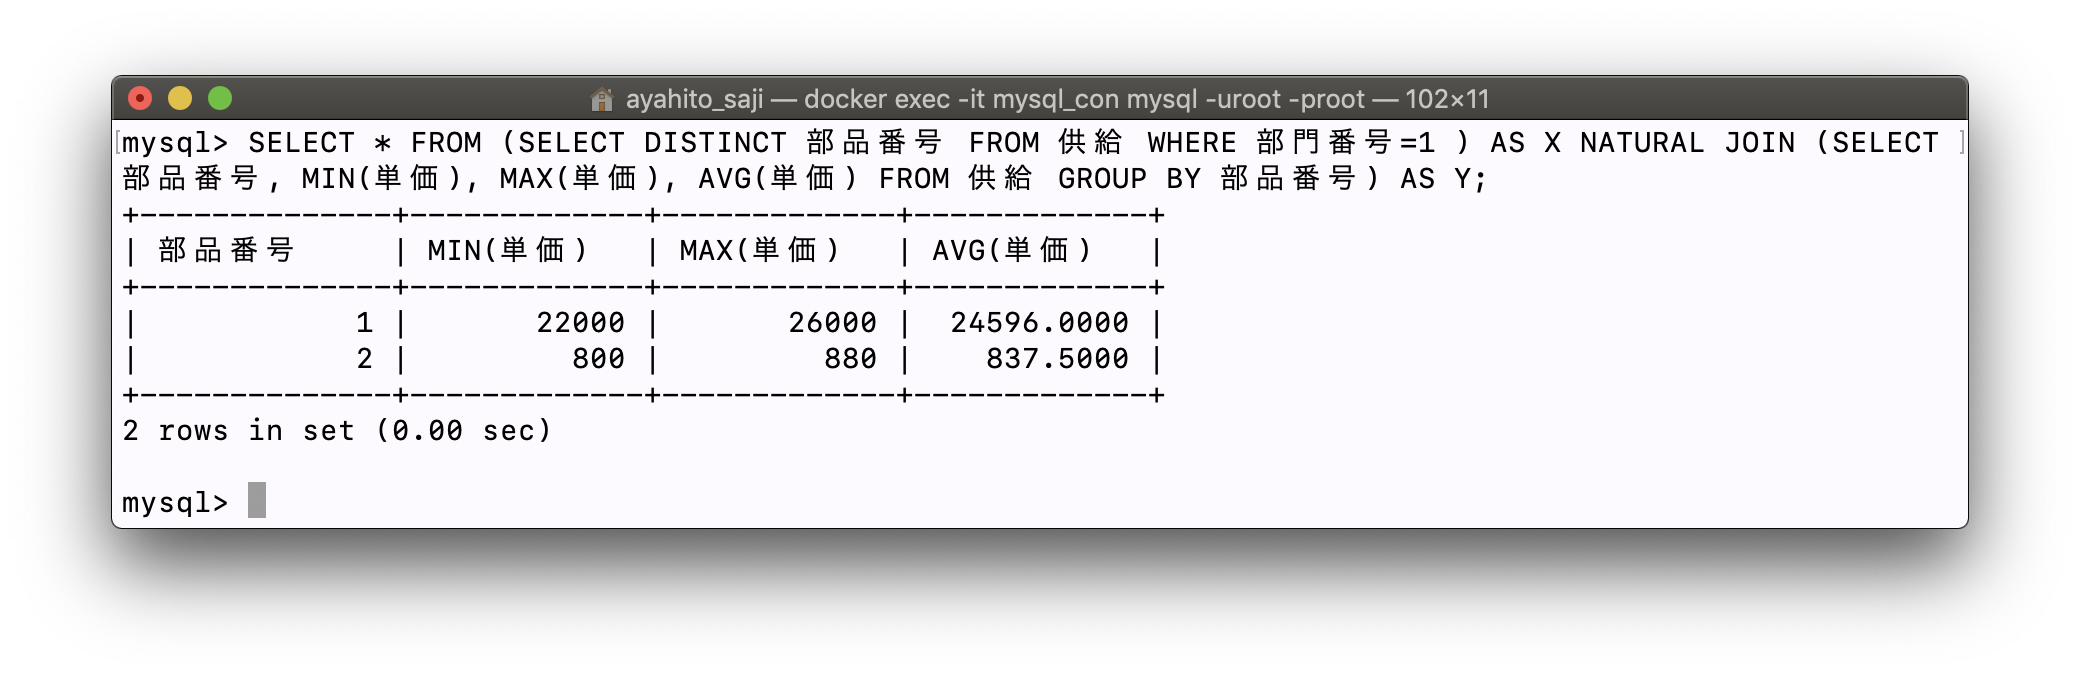
\includegraphics[width=120mm]{figures/ans10.png}
\caption{問10の実行結果}
\label{fig:ans10}
\end{center}
\end{figure}

\end{document}
